\chapter{Mathematical Formulation}
\label{chap:mipformulation}


%%%%%%%%%%%%%%%%%%%%%%%%%%%%%%%%%%%%%%%%%%%%%%%%%%%%%%%%%%%%%%%%%%%%%%%%%%%%%%%%%%

This chapter describes the current method for solving the problem, which is purely based on integer linear programming (ILP).

Solving methods can be classified as exact or non-exact methods. Exact methods try to find proven optimal solutions, but can demand unrealistic amounts of processing time whether problem size increases. Non-exact methods, basically heuristics, are generally alternatives for searching for good enough solutions in a reasonable amount of time. Development of heuristics was a consequence of the lack for many years of efficient software tools for solution of integer programming models. They have been shown to be effective in practice and have thus received much attention from researches, as mentioned by \cite{Haroldo2012}. Since the early 90's though, advances in technology have allowed mathematical programming tools development, contributing then towards the usage of exact methods.

Section ~\ref{sec:IP} introduces theory and main concepts of integer linear programming, which are fundamental in understanding the developed solving method. Further and more complete explanations about integer programming can be found at \cite{Wolsey98} and \cite{Papa98}.

Section ~\ref{sec:mathForm} introduces the mathematical model developed for the problem.

%%%%%%%%%%%%%%%%%%%%%%%%%%%%%%%%%%%%%%%%%%%%%%%%%%%%%%%%%%%%%%%%%%%%%%%%%%%%%%%%%%
\section{Integer programming}
\label{sec:IP}

A mathematical optimization problem consists of a set of inequations which together define feasible solutions for a problem and an objective function that eliminates symmetries between these solutions and guides the search for the best solution.

When both objective function and constraints are linear, then it is called \textit{Linear Programming (LP)}.

\begin{subequations}
\label{eq:LP}
\begin{align}
   \mbox{Maximize } & c \cdot x
								\\ & A \cdot x \le b
								\\ & x \in \mathbb{R}^{n}_{+}
\end{align}
\end{subequations}

where $A$ is a matrix such that $A \in \mathbb{R}^{m \times n}$, $c$ is a row vector such that $c \in \mathbb{R}^n$, $b$ is a column vector such that $b \in \mathbb{R}^m$, and $x$ is a column vector of decision variables.

Variations of a linear program are obtained when one constraints variables' domain. A \textit{Mixed Integer Program (MIP)} is a mathematical optimization in which some but not all variables are restricted to be integers. 

$$
\begin{array}{rlll}
   \mbox{Maximize} & c \cdot x & +  & h \cdot y
								\\ & A \cdot x & +  & G \cdot y \le b
								\\ & x \in \mathbb{R}^{n}_{+} &, & y \in \mathbb{Z}^{p}_{+}
\end{array}
$$

where $G$ is a matrix such that $G \in \mathbb{R}^{m \times p}$, $h$ is a row vector such that $h \in \mathbb{R}^p$, and $y$ is a column vector of integer decision variables.

When all decision variables must be integers, the program is called a \textit{Pure Integer Linear Program (IP)}:

\begin{subequations}
\label{eq:IP}
\begin{align}
   \mbox{Maximize } & c \cdot x
								\\ & A \cdot x \le b
								\\ & x \in \mathbb{Z}^{n}_{+}
\end{align}
\end{subequations}

When all decision variables are restricted to ${0,1}$ values, then we have a \textit{Binary Integer Program (BIP)}.

Very efficient methods for solving linear programs are known, with the Simplex Method being the most famous one. Because integer programs look pretty much like linear programs, it is not a surprise that linear programming theory and practice is essential in understanding and solving integer programs. Solving an integer program is far more challenging than solving its linear version though.

Since the integer set $\mathbb{Z}$ is a countable set, it is clear that every integer program has a countable number of solutions and that every bounded integer program has a countable and finite set of solutions. Thus, theoretically, these problems can be solved by enumeration. In practice, to be feasible, such approach depends on the size of the possible solutions set, and that is where difficulty stems from.

To illustrate the situation, consider a general assignment problem, where $n$ people are available to carry out $n$ jobs and each person must be assigned to carry out exactly one job. There is an one-to-one correspondence between assignments and permutations of ${1, \ldots ,n}$. Thus there are $n!$ solutions to compare. At table ~\ref{table:factorial} one can have a glimpse of what happens in this case when n grows.

\begin{table}[ht]
\caption{Combinatorial explosion of possible solutions for factorial function problems} % title of Table
\centering
\begin{tabular}{c c} 							% centered columns
\hline\hline 											% inserts double horizontal lines
$n$ & $n!$ \\ [0.5ex] 						% heading													
\hline 														% inserts single horizontal line
10 & $3.6 \cdot 10^6$ \\
100 & $9.33 \cdot 10^{157}$ \\
1000 & $4.02 \cdot 10^{2567}$ \\ [1ex] 	% [1ex] adds vertical space
\hline
\end{tabular}
\label{table:factorial} 					% is used to refer this table in the text
\end{table}


The obvious conclusion is that using complete enumeration for solving combinatorial problems, also known as \q{brute-force search} or \q{exhaustive search}, is feasible only for small values of $n$.



%%%%%%%%%%%%%%%%%%%%%%%%%%%%%%%
\subsection{Alternative formulations}

For every integer subset $X \subset \mathbb{Z}^n$ there is an infinite number of linear programs such that their feasible integer solution space is equal to $X$. Figure ~\ref{fig:linearForm} illustrates a subset $X \subset \mathbb{Z}^2$ of integer points and 3 different possible ways ($P_{1}$, $P_{2}$ and $P_{3}$) to linearly constrain the subset so that no integer point of $X$ is out of the bounded area and no integer point out of $X$ is inside the bounded area.

\begin{figure}[h]
\centering
\hfill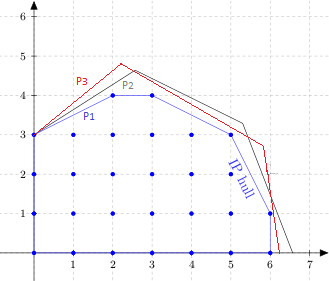
\includegraphics[scale=1.0]{figures/linearForm3.png}
\caption{Different linear formulations}
\label{fig:linearForm}
\end{figure}

Following are some useful definitions for the subject.

\paragraph{Definition}
A subset of $\mathbb{R}^{n}$ described by a finite set of linear constraints $P=\{x \in \mathbb{R}^{n}: Ax \le b\}$ is a \textit{polyhedron}.

\paragraph{Definition}
A polyhedron $P \subseteq \mathbb{R}^{n+p}$ is a \textit{formulation} for a set $X \subseteq \mathbb{Z}^{n} \times \mathbb{R}^{p}$ if and only if $X = P \cup (\mathbb{Z}^{n} \times \mathbb{R}^{p})$.

\vspace{7 mm}

Although all three formulations in figure ~\ref{fig:linearForm} are valid for definition of subset $X$, the formulation $P_{1}$ is ideal, because solving a linear program over $P_{1}$ leads to an optimal solution lying at an extreme point. Since each extreme point of $P_{1}$ is integer, it follows that the integer program is solved.

Generally speaking, given a set $X \subseteq \mathbb{R}^n$ and two formulations $P_{1}$ and $P_{2}$ for $X$, $P_{1}$ is a better formulation than $P_{2}$ if $P_{1} \subset P_{2}$. Formulation $P_{1}$ is said to be \textit{tighter} than $P_{2}$.



%%%%%%%%%%%%%%%%%%%%%%%%%%%%%%%
\subsection{Optimality and relaxation}

Regardless of the method used in the search for the optimal solution $x^*$ of an integer program, some stopping criteria is needed in the algorithm, which is equivalent to prove that a given point $x^*$ is optimal.
A pretty intuitive way is to obtain lower and upper bounds for the objective function value of the optimal solution. Hence, given an IP $$z = max\{c(x): x \in X \subseteq \mathbb{Z}^n\},$$ any algorithm will construct a decreasing sequence $$\overline{z_{1}} \ge \overline{z_{2}} \ge \ldots \overline{z_{s}} \ge z$$ of upper bounds, and an increasing sequence $$\underline{z_{1}} \le \underline{z_{2}} \le \underline{z_{t}} \le \ldots z$$ of lower bounds, and stop when $z_{s} - z_{t}$ is small enough.

Considering a maximization problem, any feasible solution provides a lower bound, also known as primal bounds. Finding upper bounds, known as dual bounds, is a different challenge. The main approach is by \q{relaxation}, the idea being to replace a difficult max (min) $IP$ by a simpler optimization problem whose optimal value is at least as large (small) as $z$.

\paragraph{Definition}
A problem (RP) $z^R = max\{f(x): x \in T \subseteq \mathbb{R}^n\}$ is a relaxation of (IP) $z = max\{c(x): x \in X \subseteq R^n\}$ if:
\begin{enumerate}
\item $X \subseteq T$, and
\item $f(x) \ge c(x)$ for all $x \in X$
\end{enumerate}

\paragraph{Proposition}
If RP is a relaxation of IP, then $z^R \ge z$.

%%%%%%%%%%%%%%
\subsubsection{Linear programming relaxation}

One way of relaxing an integer program is to enlarge the set of feasible solutions so that one optimizes over a larger set. For example, at figure ~\ref{fig:linearForm} all the three formulations $P_{1}$, $P_{2}$ and $P_{3}$ are relaxations of the original problem if we ignore the integrality constraints.

\paragraph{Definition}
For the integer program $max\{c(x): x \in P \cup \mathbb{Z}^n\}$ with formulation $P = \{x \in \mathbb{R}^{n}_{+}: Ax \le b\}$, the \textit{linear programming relaxation} is the linear program $z^{LP} = max\{cx: x \in P\}$.

However, the more the feasible solution space is enlarged, the more different the relaxed problem becomes from the original problem, which can lead to more distinct optimal solutions values for both problems. When using linear relaxations for obtaining dual bounds, this is very relevant. The more relaxed in the objective function direction is the formulation, the more distant from the actual optimal solution value will be the upper bound obtained, as illustrated in figure ~\ref{fig:objDirection}. In general, the tighter is the relaxation, the better.

\begin{figure}[h]
\centering
\hfill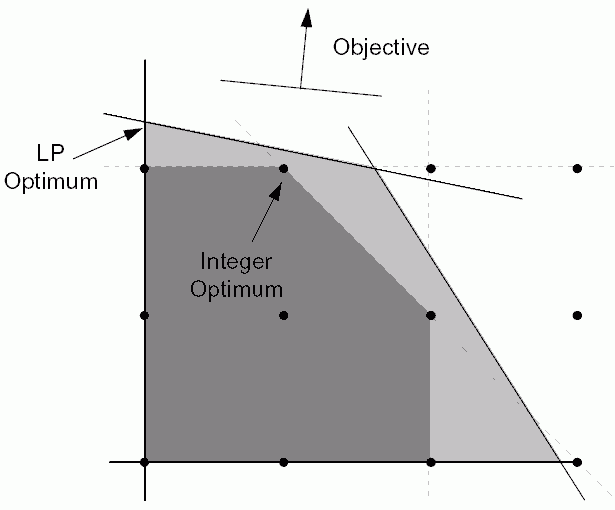
\includegraphics[scale=0.6]{figures/linearForm2.png}
\caption{Linear relaxation in the direction of objective function}
\label{fig:objDirection}
\end{figure}

Notice, though, that for a relaxation of a IP to provide an upper bound, it must be solved to optimality.

%%%%%%%%%%%%%%
\subsubsection{Duality}

Another way of finding dual bounds is through duality properties. Consider the previously introduced linear program given by \eqref{eq:LP}, called \textit{primal} problem, the following problem is referred as its \textit{dual} problem.

\begin{subequations}
\label{eq:Dual}
\begin{align}
   \mbox{Minimize } & u \cdot b
								\\ & u \cdot A \ge c
								\\ & u \in \mathbb{R}^{m}_{+}
\end{align}
\end{subequations}

Every linear program has an associated dual problem. The value of \textit{any} dual feasible solution provides an upper bound on the primal objective function value, which makes it an advantage compared to the linear relaxation. A linear programming relaxation immediately leads to a dual problem, which can then be used to obtaining dual bounds.


%%%%%%%%%%%%%%%%%%%%%%%%%%%%%%%
\subsection{Integrality gap}

Linear programming relaxation is thus a standard technique for designing approximation algorithms for optimization problems. Since such relaxation removes variables' integrality constraints, the optimal value for the relaxed maximization problem is necessarily greater than or equal to the optimal value for the original problem. The integrality gap is the maximum ratio between the solution quality of the integer program and of its relaxation. It essentially represents the inherent limits of a particular linear relaxation in approximating an integer program. Thus, the more the integral solution is improved, the smaller becomes the integrality gap.


%%%%%%%%%%%%%%%%%%%%%%%%%%%%%%%
\subsection{Branch and Bound}

Branch and bound is an implicit enumeration method for feasible solutions of combinatorial problems. Complete enumeration is inefficient and not applicable for real optimization problems, but using some knowledge on partition strategies of the problem it is possible to make intelligent decisions on whether it is necessary to explore a set of new potential solutions or about which set of potential solutions is more promising.

The \q{branch} word refers to the partitioning process of the problem and the \q{bound} refers to the decision of not exploring some set of possible new solutions (branch), avoiding exhaustive search. The bounding decisions use information of dual bounds to construct evidences of optimality and thus to eliminate branches that have proved to be unsuccessful.

Basically, for an integer linear program, the problem is decomposed and organized as a tree where each node is a subset of the solution space and a branch on that node splits the subset into mutually exclusive subsubsets. Each resulting subsubset in the partition is represented by a child of the original node. An algorithm based on linear programming is then used for calculating a dual bound on the cost of any solution in a given subset.

For further information about the branch and bound process and its strategies, see \cite{Wolsey98} and \cite{Papa98}.


%%%%%%%%%%%%%%%%%%%%%%%%%%%%%%%
\subsection{MIP Solver}

For decades limitation of computational resources was an obstacle to the development of efficient mathematical programming solvers. Since the early 90's though, advances in technology and algorithm design have allowed significant improvements in the area.

For mathematical programming there are some well-known solvers available. The most popular commercial software for optimization of (mixed integer) linear programming are IBM ILOG CPLEX Optimization Studio \fixme{conferir cplex} (\cite{Cplex}), also simply known as Cplex, and Gurobi Optimizer (\cite{Gurobi}). Both are accessible from several programming languages. CPLEX Optimization was founded in 1987, was acquired by ILOG in 1997, which was subsequently acquired by IBM in January 2009. Gurobi Optimizer was founded in 2009 by a team previously responsible for Cplex development.


This work was developed using \textit{Gurobi Optimizer version 6.0} for solving the mathematical models.



%%%%%%%%%%%%%%%%%%%%%%%%%%%%%%%%%%%%%%%%%%%%%%%%%%%%%%%%%%%%%%%%%%%%%%%%%%%%%%%%%%
%%%%%%%%%%%%%%%%%%%%%%%%%%%%%    MATH FORMULATION     %%%%%%%%%%%%%%%%%%%%%%%%%%%%
%%%%%%%%%%%%%%%%%%%%%%%%%%%%%%%%%%%%%%%%%%%%%%%%%%%%%%%%%%%%%%%%%%%%%%%%%%%%%%%%%%

\section{IP - Assignment Formulation for the Timetabling Problem}
\label{sec:mathForm}

The general process of formulating an integer program can be organized in three steps:

\begin{enumerate}
\item Define what appear to be the necessary variables.
\item Use these variables to define a set of constraints so that the feasible points correspond to feasible solutions to the problem.
\item Use these variables to define the objective function.
\end{enumerate}

Usually the need of auxiliary variables arises while formulating constraints, which gives an iterative feature to the process until a consistent model is reached.

Next subsections introduce the notation used in the mathematical model, which includes data sets, general data and model variables, and the formulation, which includes a multi-objective function and all constraints.

%%%%%%%%%%%%%%%%%%%%%%%%%%%%%%%%%%%%%%%%%%%%%%%%%%%%%%%%%%%%%%%%%%%%%%%%%%%%%%%%%%

\subsection{Notation}

%%%%%%%%%%%%%%%%%%%%%%%%%%%%%%%%%%%%%%%%%%
\subsubsection{Sets}

\begin{itemize}
\item $Al$ - Set of students. Elements of $Al$ are called $a$.
\item $C$ - Set of majors. Elements of $C$ are called $c$.
\item $D$ - Set of courses. Elements of $D$ are called $d$.
\item $Dm$ - Set of courses for which lessons are shareable between different classes, that is, lessons can be \textit{merged}. Elements of $D$ are called $d$.
\item $D_{a}$ - Set of courses required by student $a$.
\item $H$ - Set of time slots. Elements of $H$ are called $h$.
\item $H_{f}$ - Set of time slots of session of day $f$. Elements are called $h$.
\item $I_{d}$ - Set of sections of a course $d$. Elements of $I_{d}$ are called $i$.
\item $O$ - Set of majors offers. Elements of $O$ are called $oft$.
\item $U$ - Set of blocks. Elements of $U$ are called $u$.
\item $S_{u}$ - Set of classrooms of block $u$. Elements of $S_{u}$ are called $s$.
\item $T$ - Set of weekdays. Elements of $T$ are called $t$.
\item $U$ - Set of blocks. Elements of $U$ are called $u$.
\item $SL$ - Set of calenders. Elements of $SL$ are called $sl$.
\item $P$ - Set of all professors. Elements of $P$ are called $p$.
\item $P_{prior}$ - Set of all professors with some priority $prior$. Elements of $P$ are called $p$.
\end{itemize}

%%%%%%%%%%%%%%%%%%%%%%%%%%%%%%%%%%%%%%%%%%
\subsubsection{Model Data}

\begin{itemize}
\item $Cap_{s}$ - Capacity of classroom $s$.
\item $nCreds_{d}$ - Total of credits of course $d$.
\item $duration_{h}$ - Total of minutes of time slot $h$.
\item $duration_{hi,hf}$ - Total of minutes from the beginning of time slot $hi$ to the end of time slot $hf$.
\item $M$ - called \q{big M}, it is a large enough value that depends on the constraint it is applied to.
\item $N_{d,k,t}$ - number of credits for course $d$ at day $t$ of credits split rule $k$.
\item $NCH_{d,hi,hf}$ - number of credits for course $d$ from time slot $hi$ to time slot $hf$.
\item $MinSize$ - minimum number of students required for offering a class.
\item $delta_{t,f}$ - maximum of idle time allowed at phase $f$ of day $t$ for a professor. Used only for gap-constraints, usually is the average sum of intervals at phase $f$ of day $t$ of calenders.
\item $pv$ - Unique virtual professor, to be used whenever the set of real professors is not enough for demand satisfaction.
\item $MinCredsDia_{a,t}$ - minimum number of credits expected for student $a$ at day $t$.
\item $MaxNrCredsDay_{p,t}$ - maximum number of credits available at day $t$ of professor $p$.
\item $Time_{u1,u2}$ - minimum number of minutes necessary for moving between blocks $u1 \in U$ and $u2 \in U$.
\item $MaxGapBetweenSessions$ - maximum idle interval between 2 consecutive day sessions that a professor is assigned to. It is used to avoid situations like a professor being assigned to a class early in the morning and then another just late in the afternoon, with a big idle inbetween interval. A reasonable value is around 170 minutes.
\end{itemize}

%%%%%%%%%%%%%%%%%%%%%%%%%%%%%%%%%%%%%%%%%%
\subsubsection{Variables}

All possible variables used in the model are following described. The need of some of them depends on considering or not some constraints, in the sense that the more restrictions and requirements exist, the more auxiliary variables are need.

\begin{itemize}
\item $v_{a,i,d,s,t,hi,hf}$ - binary variable, indicates if student $a$ is assigned to a class of section $i$ of course $d$, at classroom $s$, from time slot $hi$ to time slot $hf$ of day $t$. 
\item $x_{i,d,u,s,hi,hf,t}$ - binary variable, indicates if section $i$ of course $d$ is assigned to classroom $s$ from time slot $hi$ to time slot $hf$ of day $t$. 
\item $z_{i,d}$ - binary variable, indicates if section $i$ of course $d$ is offered. 
\item $o_{i,d,s}$ - binary variable, indicates if section $i$ of course $d$ is offered at classroom $s$. 
\item $fd_{d,a}$ - binary slack variable, indicates if student $a$ has his request for course $d$ not satisfied.
\item $m_{d,i,k}$ - binary variable, indicates if a credits split rule $k$ was chosen for section $i$ of course $d$.
\item $s_{i,d,a}$ - binary variable, indicates if student $a$ is assigned to section $i$ of course $d$.
\item $k_{p,i,d,u,h,t}$ - binary variable, indicates if professor $p$ teaches to section $i$ of course $d$ at block $u$ at time slot $h$ and day $t$.
\item $y_{p,i,d}$ - binary variable, indicates if professor $p$ is assigned to section $i$ of course $d$.
\item $hip_{p,t,f}$ - integer variable, indicates the time in minutes of the first time slot assigned to professor $p$ at session $f$ of day $t$. For example, if the first class assigned to $p$ on $t=Monday$ and $f=morning$ starts at 9:30 am, then $hip_{p,t,f}=9\cdot 60 + 30 = 570$.
\item $hfp_{p,t,f}$ - integer variable, indicates the time in minutes of the end of the last time slot assigned to professor $p$ at session $f$ of day $t$.
\item $fpgap_{p,t,f}$ - integer slack variable, indicates the gap in session $f$ of day $t$ of professor $p$'s schedule.
\item $fcad_{a,t}$ - integer slack variable, indicates the number of credits bellow the expected assigned to student $a$ at day $t$.
\item $begin_{a,t,h}$ - binary variable, indicates if first class of student $a$ at day $t$ begin at time $h$.
\item $end_{a,t,h}$ - binary variable, indicates if last class of student $a$ at day $t$ begin at time $h$.
\item $at_{a,t}$ - binary variable, indicates if student $a$ has classes at day $t$.
\item $uu_{p,t,u}$ - binary variable, indicates if professor $p$ has classes at day $t$ in block $u$.
\item $desloc_{p,t,u1,u2}$ - binary variable, indicates whether professor $p$ has classes at day $t$ in block $u1$ and in block $u2$. In practice, it identifies that at least one displacement is made between the both blocks in the day.
\item $ptf_{p,t,f}$ - binary variable, indicates if professor $p$ has classes at session $f$ of day $t$.
\item $pt_{p,t}$ - binary variable, indicates if professor $p$ has classes at day $t$.


\end{itemize}


%%%%%%%%%%%%%%%%%%%%%%%%%%%%%%%%%%%%%%%%%%%%%%%%%%%%%%%%%%%%%%%%%%%%%%%%%%%%%%%%%%
%%%%%%%%%%%%%%%%%%%%%%%%%%%%%%%%%%%%%%%%%%%%%%%%%%%%%%%%%%%%%%%%%%%%%%%%%%%%%%%%%%

\subsection{Formulation}


\subsubsection{Objective function}

The following general objective function includes all possible minimization goals, with their subjective weights to be decided according to the scenario or the user preferences. Further alternatives of how to handle disparate goals are discussed at section ~\ref{sec:goal}.

$$
\begin{array}{rl}
   \mbox{MIN} &
			\lambda \cdot \sum\limits_{a \in A}\sum\limits_{d \in D} \cdot fd_{d,a}
      \\
      &
       + \beta \cdot \sum\limits_{a \in A} \sum\limits_{t \in T} fcad_{a,t}
      \\
      &      
      + \epsilon \cdot \sum\limits_{p \in P} \sum\limits_{t \in T} \sum\limits_{f \in F} fpgap_{p,t,f}
			\\
			&
			+ \sigma \cdot \sum\limits_{p \in P} \sum\limits_{t \in T} \sum\limits_{u1 \in U} \sum\limits_{u2 \in U} Time_{u1,u2} \cdot desloc_{p,t,u1,u2}
      \\
      &
      + \gamma \cdot \sum\limits_{i \in I_{d}} \sum\limits_{d \in D} y_{pv,i,d}
      \\
      &
      + \alpha \cdot \sum\limits_{p \in P} \sum\limits_{t \in T} pt_{p,t}
      \\
      &
      + \alpha \cdot \sum\limits_{p \in P} \sum\limits_{t \in T} \sum\limits_{f \in F} ptf_{p,t,f}
      
\end{array}
$$


%%%%%%%%%%%%%%%%%%%%%%%%%%%%%%%%%%%%%%%%%%%%%%%%%%%%%%%%%%%%%%%%%%%%%%%%%%%%%%%%%%
%%%%%%%%%%%%%%%%%%%%%%%%%%%%%%%%%%%%%%%%%%%%%%%%%%%%%%%%%%%%%%%%%%%%%%%%%%%%%%%%%%


\subsubsection{Assigns 'v' to 'x' and ensures classroom capacity}
\begin{eqnarray}
\sum\limits_{a \in A} v_{a,i,d,s,t,hi,hf}  \le Cap_{s} \cdot x_{i,d,s,t,hi,hf} \nonumber \qquad 
\\
\forall d \in D \quad
\forall i \in I_{d} \quad 
\forall s \in S \quad
\forall t \in T \quad 
\forall hi \in H \quad 
\forall hf \in H \nonumber
\end{eqnarray}

\subsubsection{Assigns the classroom of a section to variable 'o'}
\begin{eqnarray}
M \cdot o_{i,d,s}  \geq \sum\limits_{t \in T}\sum\limits_{hi \in H}\sum\limits_{hf \in H} x_{i,d,s,t,hi,hf}  \nonumber \qquad 
\\
\forall d \in D \quad
\forall i \in I_{d} \quad
\forall u \in U \quad
\forall s \in S_{u} \nonumber
\end{eqnarray}

\subsubsection{Ensures single classroom per course section}
\begin{eqnarray}
\sum\limits_{u \in U} \sum\limits_{s \in S_{u}} o_{i,d,s} = z_{i,d}  \nonumber \qquad 
\forall d \in D \quad
\forall i \in I_{d} \quad
\end{eqnarray}

\subsubsection{No overlapping in classroom's timetable}
\begin{eqnarray}
\sum\limits_{i \in I_{d}} \sum\limits_{d \in D} \sum\limits_{hi \in H_{d}} \sum_{\substack {hf \in H_{d} \\ hi\le hf}} x_{i,d,s,t,hi,hf}  \leq  1  \nonumber \qquad 
\\
\forall u \in U \quad
\forall s \in S_{u} \quad
\forall t \in T \quad
\forall h \in H \quad (hi,hf)\text{ overlaps }h \nonumber
\end{eqnarray}

\subsubsection{Tries to satisfy each student requirement}
\begin{eqnarray}
\sum\limits_{i \in I_{d}} s_{i,d,a} + fd_{d,a} = 1  \nonumber \qquad 
\forall a \in Al \quad
\forall d \in D_{a}
\end{eqnarray}

\subsubsection{Assigns student's course section to lessons, while ensures course section's total number of credits}
\begin{eqnarray}
nCreds_{d} \cdot s_{i,d,a} = \sum\limits_{s \in S}\sum\limits_{t \in T}\sum\limits_{hi \in H}\sum\limits_{hf \in H} NHC_{d,hi,hf} \cdot v_{a,i,d,s,t,hi,hf} \nonumber \qquad 
\forall a \in A \quad
\forall i \in I_{d} \quad
\forall d \in D_{a}
\end{eqnarray}

\subsubsection{Links variables x and variable z, while ensures course section's total number of credits}
\begin{eqnarray}
\sum\limits_{s \in S}\sum\limits_{t \in T}\sum\limits_{hi \in H}\sum\limits_{hf \in H} NHC_{d,hi,hf} \cdot x_{i,d,s,t,hi,hf} = nCreds_{d} \cdot z_{i,d} \nonumber \qquad
\forall i \in I_{d} \quad
\forall d \in D \quad
\end{eqnarray}

\subsubsection{Avoids classes overlapping at student timetable}
\begin{eqnarray}
\sum\limits_{u \in U} \sum\limits_{s \in S_{u}} \sum\limits_{i \in I_{d}} \sum\limits_{d \in D_{a}} \sum\limits_{hi \in H_{d}} \sum_{\substack {hf \in H_{d} \\ hi\le hf \\ (hi,hf)\mbox{ overlaps }h}} v_{a,i,d,s,hi,hf,t}  \leq  1  \nonumber \qquad 
\\
\forall a \in A \quad
\forall t \in T \quad
\forall h \in H_{d} \nonumber
\end{eqnarray}

\subsubsection{Single lesson for each course section per day}
\begin{eqnarray}
\sum\limits_{u \in U} \sum\limits_{s \in S_{u}} \sum\limits_{hi \in H_{d}} \sum_{\substack {hf \in H_{d} \\ hi\le hf}} x_{i,d,s,hi,hf,t}  \leq  1  \nonumber \qquad 
\forall d \in D \quad
\forall i \in I_{d} \quad
\forall t \in T 
\end{eqnarray}


%%%%%%%%%%%%%%%%%%%%%%%%%%%%%%%%%%%%%%%%%%%%%%%%%%%%%%%%%%%
% 		EXPECTED NUMBER OF CREDITS FOR EACH STUDENT PER DAY

\subsubsection{Try to ensure the expected number of credits for each student per day}
\begin{eqnarray}
\sum\limits_{i \in I_{d}} \sum\limits_{d \in D_{a}} \sum\limits_{s\in S} \sum\limits_{hi\in H} \sum\limits_{hf\in H} nCreds_{d} \cdot v_{a,i,d,s,t,hi,hf} + fcad_{a,t} \ge MinCredsDia_{a,t} \nonumber \qquad
\forall a \in A \quad
\forall t \in T
\end{eqnarray}


%%%%%%%%%%%%%%%%%%%%%%%%%%%%%%%%%%%%%%%%%%%%%%%%%%%%%%%%%%%
% 					CREDITS SPLIT RULES
\subsubsection{Credits split rules}

\paragraph{Credits split rule for each course section}
\begin{eqnarray}
\sum\limits_{u \in U} \sum\limits_{s \in S_{u}} \sum\limits_{hi \in H_{d}} \sum_{\substack {hf \in H_{d} \\ hi\le hf}}
 NCH_{d,hi,hf} \cdot x_{i,d,u,s,hi,hf,t} = \sum\limits_{k \in K_{d}}N_{d,k,t} \cdot m_{d,i,k} \nonumber \qquad 
\\
\forall d \in D \quad
\forall i \in I_{d} \quad
\forall t \in T \nonumber
\end{eqnarray}

\paragraph{Single credits split rule for each course section}
\begin{eqnarray}
\sum\limits_{k \in K_{d}} m_{d,i,k} = z_{i,d} \nonumber \qquad 
\forall d \in D \quad
\forall i \in I_{d}
\end{eqnarray}


%%%%%%%%%%%%%%%%%%%%%%%%%%%%%%%%%%%%%%%%%%%%%%%%%%%%%%%%%%%
% 				GAPS IN STUDENT'S TIMETABLE
\subsubsection{Student's gaps prohibition}
\label{constrStudentGap}

Following, auxiliary variables necessary for preventing gaps in student's timetable are consistently set.

\paragraph{Sets if student $a$ has classes at day $t$ (variable $at_{a,t}$)}
\begin{eqnarray}
M \cdot at_{a,t} \ge \sum\limits_{i \in I_{d}} \sum\limits_{d \in D_{a}} \sum\limits_{u \in U} \sum\limits_{s \in S_{u}} \sum\limits_{hi \in H_{d}} \sum_{\substack {hf \in H_{d} \\ hi\le hf}} v_{a,i,d,u,s,hi,hf,t} \nonumber \qquad 
\forall a \in A \quad
\forall t \in T
\end{eqnarray}

\paragraph{Sets beginning time of classes for student $a$ at day $t$ (variable $begin_{a,t,h}$)}
\begin{eqnarray}
begin_{a,t,h} = \sum\limits_{v} v_{a,t,hi} - \sum\limits_{h'\le h} begin_{a,t,h'} + \sum\limits_{h'\le h} end_{a,t,h'} \nonumber \qquad
\forall a \in A \quad
\forall t \in T \quad
\forall h \in H
\end{eqnarray}

\paragraph{Sets ending time of classes for student $a$ at day $t$ (variable $end_{a,t,h}$)}
\begin{eqnarray}
end_{a,t,h} = \sum\limits_{v} v_{a,t,hi} - \sum\limits_{h'\ge h} end_{a,t,h'} + \sum\limits_{h'\ge h} begin_{a,t,h'} \nonumber \qquad
\forall a \in A \quad
\forall t \in T \quad
\forall h \in H
\end{eqnarray}

\paragraph{Uniqueness of student's last class of the day}
\begin{eqnarray}
\sum\limits_{h\in H} end_{a,t,h} = at_{a,t} \nonumber \qquad
\forall a \in A \quad
\forall t \in T
\end{eqnarray}

\paragraph{Uniqueness of student's first class of the day}
\begin{eqnarray}
\sum\limits_{h\in H} begin_{a,t,h} = at_{a,t} \nonumber \qquad
\forall a \in A \quad
\forall t \in T
\end{eqnarray}


Next, gaps in student timetable are prevented. Unlike professors similar restriction, students can not have idle times, and therefore these are hard constraints and there are no slack variables.

\paragraph{Prohibits gap in student timetable}
\begin{eqnarray}
\sum\limits_{i\in I_{d}} \sum\limits_{d\in D} \sum\limits_{s\in S} \sum\limits_{hf\in H} v_{a,i,d,s,t,hi+,hf} = 
\sum\limits_{i\in I_{d}} \sum\limits_{d\in D} \sum\limits_{s\in S} \sum\limits_{hf\in H} v_{a,i,d,s,t,hi-,hf} - end_{a,t,hi-} + begin_{a,t,hi+} \nonumber \qquad
\\
\forall a \in A \quad
\forall t \in T \quad
\forall hi+ \in H \quad hi- \in H \mbox{ s.t. hi- + 1 = hi+} \nonumber
\end{eqnarray}


%%%%%%%%%%%%%%%%%%%%%%%%%%%%%%%%%%%%%%%%%%%%%%%%%%%%%%%%%%%
% 					PROFESSORS ASSIGNMENT
\subsubsection{Professors assignment}

The following constraints, responsible for assigning professors to classes, involve both real professors and the virtual teaching resource $pv$.

\paragraph{No overlapping in professor's timetable}
\begin{eqnarray}
\sum_{ \substack {dti,dtf \in Dt \\ dt \in [dti,dtf)} } \sum\limits_{i \in I_{d}} \sum\limits_{d \in D} \sum\limits_{u \in U} k_{p,i,d,u,t,dti,dtf} \le 1 \nonumber \qquad
\forall p \in P \cup \{pv\} \quad
\forall t \in T \quad
\forall dt \in Dt
\end{eqnarray}

\paragraph{Assigns professor to class (sets variable k)}
% Part 1
\begin{eqnarray}
\sum_{ \substack {hi,hf \in H \\ dti \in [hi,hf)} } \sum\limits_{s\in S_{u}} x_{i,d,s,t,hi,hf} \le k_{p,i,d,u,t,dti} + ( 1 - y_{p,i,d} ) \nonumber \qquad
\\
\forall i \in I \quad
\forall d \in D \quad
\forall u \in U \quad
\forall p \in P \cup \{pv\} \quad
\forall t \in T \quad
\forall dti \in Dt \nonumber
\end{eqnarray}
% Part 2
\begin{eqnarray}
\sum_{ \substack {hi,hf \in H \\ dti \in [hi,hf)} } \sum\limits_{s\in S} x_{i,d,s,t,hi,hf} \le \sum\limits_{u\in U} \sum\limits_{p \in P \cup \{pv\}} k_{p,i,d,u,t,dti} \nonumber \qquad
\\
\forall i \in I \quad
\forall d \in D \quad
\forall t \in T \quad
\forall dti \in Dt \nonumber
\end{eqnarray}
	
\paragraph{Assigns professor to class (sets variable y)}
\begin{eqnarray}
\sum\limits_{u \in U} \sum\limits_{t \in T} \sum\limits_{h \in H} k_{p,i,d,u,t,h} = nCreds_{d} \cdot y_{p,i,d} \nonumber \qquad
\forall i \in I \quad
\forall d \in D \quad
\forall p \in P \cup \{pv\}
\end{eqnarray}	
	
\paragraph{Assigns a single professor to each course section}
\begin{eqnarray}
\sum\limits_{p\in P \cup \{pv\}} y_{p,i,d} = z_{i,d} \nonumber \qquad
\forall i \in I \quad
\forall d \in D
\end{eqnarray}	


%%%%%%%%%%%%%%%%%%%%%%%%%%%%%%%%%%%%%%%%%%%%%%%%%%%%%%%%%%%
%						PROFESSOR DISPLACEMENT
\subsubsection{Professor's displacement}
\label{constrProfessorDisplac}

Here quality constraints related to displacement of real professors along the week and in a day are considered.


\paragraph{Ensures enough time for displacement between blocks in the same day}
\begin{eqnarray}
\sum\limits_{i \in I_{d}} \sum\limits_{d \in D} k_{p,i,d,u1,t,h1} + \sum\limits_{i\in I_{d}} \sum\limits_{d \in D} k_{p,i,d,u2,t,h2} \le 1 \nonumber
\\
\forall p \in P \quad
\forall t \in T \quad
\forall u1 \in U \quad
\forall u2 \in U \quad
\forall h1 \in H \quad
\forall h2 \in H \nonumber
\end{eqnarray}	
\textit{s.t. time between ending of h1 and beginning of h2 is less than displacement time between u1 and u2}.

\paragraph{Ensures the maximum of 1 displacement for each professor in the same day}
\begin{eqnarray}
\sum\limits_{i\in I_{d}} \sum\limits_{d \in D} k_{p,i,d,u1,t,h1} + \sum\limits_{i\in I_{d}} \sum\limits_{d \in D} k_{p,i,d,u2,t,h2} + \sum\limits_{i\in I_{d}} \sum\limits_{d \in D} k_{p,i,d,u3,t,h3} \le 2 \nonumber
\\
\forall p \in P \quad
\forall t \in T \quad
\forall u2 \in U \quad
\forall h2 \in H \nonumber
\\
\mbox{s.t. }u1 \neq u2 \qquad u3 \neq u2 \qquad h1<h2 \qquad h3>h2 \nonumber
\end{eqnarray}

\paragraph{Identifies if the professor teaches in a block at the day}
\begin{eqnarray}
\sum\limits_{i\in I_{d}} \sum\limits_{d \in D} \sum\limits_{h \in H} k_{p,i,d,u,t,h} \le MaxNrCredsDay_{p,t} \cdot uu_{p,t,u} \nonumber \qquad
\\
\forall p \in P \quad
\forall t \in T \quad
\forall u \in U \quad \nonumber
\end{eqnarray}

\paragraph{Constraints the maximum number of blocks assigned to the professor at the day}
\begin{eqnarray}
\sum\limits_{u \in U} uu_{p,t,u} \le 2 \nonumber \qquad
\forall p \in P \quad
\forall t \in T \quad \nonumber
\end{eqnarray}

\paragraph{Identifies displacements in the day of the professor}
\begin{eqnarray}
uu_{p,t,u1} + uu_{p,t,u2} \le 1 + desloc_{p,t,u1,u2} \nonumber \qquad
\\
\forall p \in P \quad
\forall t \in T \quad
\forall u1 \in U \quad
\forall u2 \in U \quad \mbox{s.t. }u1 \neq u2 \nonumber
\end{eqnarray}


\paragraph{Limits the maximum of 2 big displacements for each professor along the week}
\begin{eqnarray}
\sum\limits_{t \in T} \sum\limits_{u1 \in U} \sum_{\substack {u2 \in U \\ \norm{u1 u2} \ge 50}} desloc_{p,t,u1,u2} \le 2 \nonumber \qquad
\forall p \in P \quad \nonumber
\end{eqnarray}



%%%%%%%%%%%%%%%%%%%%%%%%%%%%%%%%%%%%%%%%%%%%%%%%%%%%%%%%%%%
%						GAPS IN PROFESSOR'S TIMETABLE									% 							 
\subsubsection{Professor's gaps avoidance}
\label{constrProfessorGap}

Next, variables $hip_{p,t,f}$ and $hfp_{p,t,f}$ are set. We draw attention to the fact of these variables being strictly set, i.e., less and greater inequality constraints are used per variable, resulting in an implicit equality constraint. Consequently, they do not depend on an objective function, which is important when it has conflicting goals. \fixme{Exemplify!} \fixme{exception when the professor is not assigned at the day}

\paragraph{Sets variable $hip_{p,t,f}$}
\begin{eqnarray}
hip_{p,t,f} \geq m(dt) \cdot ( 1 - \sum\limits_{k \in K_{dti<dt}} k_{p,t,dti} ) \nonumber \qquad
\forall p \in P \quad
\forall t \in T \quad
\forall f \in F \quad
\forall dt \in Dt_{f}
\end{eqnarray}
\begin{eqnarray}
hip_{p,t,f} \leq m(dt) + M \cdot ( 1 - \sum\limits_{k} k_{p,t,dti} ) \nonumber \qquad
\forall p \in P \quad
\forall t \in T \quad
\forall f \in F \quad
\forall dti \in Dt_{f}
\end{eqnarray}

\paragraph{Sets variable $hfp_{p,t,f}$}
\begin{eqnarray}
hfp_{p,t,f} \geq \sum\limits_{k} m(dt) \cdot k_{p,t,dtf} \nonumber \qquad
\forall p \in P \quad
\forall t \in T \quad
\forall f \in F \quad
\forall dtf \in Dt_{f}
\end{eqnarray}
\begin{eqnarray}
hfp_{p,t,f} \leq m(dt) + M \cdot ( \sum\limits_{k \in K_{dtf>dt}} k_{p,t,dtf} ) \nonumber \qquad
\forall p \in P \quad
\forall t \in T \quad
\forall f \in F \quad
\forall dt \in Dt_{f}
\end{eqnarray}

Next, gaps in professor timetable are controlled. The usage of the slack variable $fpgap_{p,t,f}$ indicates the amount of idle time in session $f$ of day $t$ for professor $p$. The reduce of professors idle time is achieved through minimization of these slack variables in objective function.

\paragraph{Prohibits gap in each session of day in professor timetable}
\begin{eqnarray}
\sum\limits_{k \in K_{h \in H_{f}}} duration_{h} \cdot k_{p,t,h} + delta_{f,t} + fpgap_{p,t,f} \geq hfp_{p,t,f} - hip_{p,t,f} \nonumber \qquad
\\
\forall p \in P \quad
\forall t \in T \quad
\forall f \in F \quad \nonumber
\end{eqnarray}



%%%%%%%%%%%%%%%%%%%%%%%%%%%%%%%%%%%%%%%%%%%%%%%%%%%%%%%%%%%
%						COMPACTING PROFESSOR'S TIMETABLE							% 							 
\subsubsection{Professor's timetable compactness}
\label{constrProfCompact}

Besides constraints introduced at ~\ref{constrProfessorGap}, specific for avoiding gaps in each session of a professor's day, here further quality constraints related to compactness of real professors' timetable along the week and in a day are considered.


\paragraph{Sets if a session of day is assigned for the professor}
\begin{eqnarray}
M \cdot ptf_{p,t,f} \ge \sum\limits_{d \in D}\sum\limits_{i \in I_{d}}\sum\limits_{u \in U}\sum\limits_{h \in H_{f}} k_{p,i,d,u,t,h} \nonumber \qquad
\\
\forall p \in P \quad
\forall T \in T \quad
\forall f \in F \nonumber
\end{eqnarray}

\paragraph{Sets the number of days of the week assigned to each professor}
\begin{eqnarray}
M \cdot pt_{p,t} \ge \sum\limits_{f \in F} ptf_{p,t,f} \nonumber \qquad
\forall p \in P \quad
\forall t \in T \nonumber
\end{eqnarray}

\paragraph{Prohibits big gaps between assigned sessions of the day}
\begin{eqnarray}
hip_{p,t,f} - hfp_{p,t,f-1} \le (MaxGapBetweenSessions + M \cdot(2 - ptf_{p,t,f} - ptf_{p,t,f-1}))  \nonumber \qquad
\\
\forall p \in P \quad
\forall t \in T \quad
\forall f \in F \quad \nonumber
\end{eqnarray}



%%%%%%%%%%%%%%%%%%%%%%%%%%%%%%%%%%%%%%%%%%%%%%%%%%%%%%%%%%%%%%%%%%%%%%%%%%%%%%%%%%%%%%%%%%
